\chapter{Aufgabe 3}

\section{Teil 1}

\textit{Ein UHF-RFID-Reader kann nicht nur einzelne, sondern viele Transponder gleichzeitig erfassen (Pulkerfassung, engl. Bulk Reading). Wie
funktioniert das - es müssten dazu die einzelnen Transponder voneinander unterschieden werden?}\\

\noindent
Das \textit{Bulk Reading} sieht sich u.a. zwei Herausforderungen gegenüber:

\begin{enumerate}
    \itemsep0.5em
    \item Zuverlässiges \textit{Lesen} von RFID-Tags in Bereichen mit einer hohen Anzahl gleichzeitig antwortender Tags\footnote{
    siehe hierzu auch Teilaufgaben~\ref{sec:2_4}.
    }
    \item Zuverlässiges \textit{Identifizieren} der Signale zur eindeutigen Zuordnung zu den einzelnen Tags
\end{enumerate}

\noindent
Damit dies funktioniert, kann der \textbf{RSSI} (\textit{Radio Signal Strength Indicator}) verwendet werden, der die gemessene Feldstärkewerte beim Lesen meldet (vgl.~\cite[136]{ES5}) und so dem Leser Auskunft über ungefähre Position und Abstand des Transponders liefert.\\
\textit{Finkenzeller} stellt in~\cite[194]{Fin10} verschiedene Verfahren vor, um das Problem von Signalkollisionen in den Griff zu bekommen, darunter \textit{SDMA} (\textit{Space Division Multiple Access}), bei der die Reichweite einzelner Leser verringert wird, aber mehrere Leser in einem Feld angeordnet sind, um einen bestimmten Bereich zu erfassen - die Leser innerhalt dieser Felder werden nacheinander aktiviert, um Interferenzen zu vermeiden.\\
Protokolle, die auf \textit{TDMA} (\textit{Time Domain Multiple Access}) basieren, spezifizieren u.a. das ``Stummschalten`` des Transponders, sobald der Leser ihr Signal erkannt hat.\\
Ein Verfahren, das auf \textit{TDMA} aufbaut, ist das \textit{Slotted ALOHA}-Verfahren, bei denen der Leser Zeitbereiche (``time slots``) vorgibt, in denen er Signale erwartet.
Die Transponder wählen daraufhin \textit{zufällig} einen Slot aus, in dem sie ihr Signal senden, um mögliche Kollisionen durch gleichzeitiges Senden zu vermeiden:

\blockquote[{\cite[201]{Fin10}}]{
    ``In this procedure, transponders may only begin to transmit data
    packets at defined, synchronous points in time (slots). The synchronisation of all transponders
    necessary for this must be controlled by the reader. This is therefore a stochastic, interrogator-driven
    TDMA anticollision procedure.``
}

\section{Teil 2)}

\textit{Warum sollte ein UHF-RFID-Reader mehrere Antennenausgänge besitzen, die geschaltet werden können. Es sollte doch ausreichen, die
Antennen parallel an einen Ausgang zu schalten?}\\

\noindent
Das Schalten einzelner Antennenausgänge erlaubt die Anwendung unterschiedlicher Anti-Kollisionsverfahren zur \textit{zeitlichen} und \textit{räumlichen} Trennung von Signalen, wie in der vorherigen Aufgabe am Beispiel \textit{SDMA} erwähnt.
Das Parallelschalten von Antennen würde eine gleichzeitige Erfassungen mehrere Signale bedeuten, was mit hoher Wahrscheinlichkeit durch die Überlappung mehrerer Messzonen zu ungenauen Ergebnissen führt.

\section{Teil 3)}

\textit{Ein Gabelstapler mit UHF-RFID-Reader und einer Antenne fährt auf
einen Stapel mit Paketen zu. die Pakete sind mit UHF-Transpondern
ausgerüstet. Wie könnten dicht vor dem Gabelstapler liegende Pakete
von weiter weg liegenden unterschieden werden?}\\

\noindent
Durch die Einbeziehung des bereits erwähnten \textit{Received Signal Strength Indicators} kann über die gemeldete Feldstärke eine grobe Abschätzung erfolgen, welche Transponder sich näher an der Antenne befinden.

\section{Teil 4)}

\textit{In Ihrer Firma gibt es einen Parkplatz für Firmenangehörige. Der
Parkplatz ist mit einer Parkschranke gesichert. Wie könnte mit
Hilfe von RFID erreicht werden, dass einfahrende PKWs langsam
auf die geschlossene Schranke zufahren und ohne anzuhalten durch
die sich hebende Schranke eingelassen werden?\\Welche Frequenz würden Sie für die RFID-Chips wählen?}\\

\noindent
An dem PKW kann ein RFID-Tag angebracht werden, der von der Schrankensteuerung gelesen wird.
Bei einer zuverlässigen Erfassung des Signals startet der Öffnungsvorgang (nach Abgleich der zur Einfahrt zugelassenen Fahrzeuge).
Unter Berücksichtigung der geltenden Sicherheitsvorschriften beginnt der Schließvorgang bei Signalverlust.
Wird der RSSI berücksichtigt, könnte die Geschwindigkeit, mit der die Schrankenmechanik arbeitet, auch unter Einbeziehung der gemessenen Feldstärke dynamisch angepasst werden.\\
Damit der Öffnungs-/Schließvorgang möglichst sanft gesteuert wird, könnte für das System ein UHF-RFID-Tag mit einem Frequenzbereich von 865MHz gewählt werden, damit rechtzeitig geöffnet und die Schranke \textit{nicht zu früh} geschlossen wird.
Sollte der Schliessvorgang über eine Lichtschranke angestoßen werden, könnte je nach Montageposition auch ein HF-Tag mit 13.56 MHz ausreichend sein.
Je nach Motorhaubendimension/Wagenlänge wäre man mit einem höheren Frequenzbereich auf der sicheren Seite.

\section{Teil 5)}

\textit{In Neustadt sollen die Menschen unterstützt werden, die mithelfen, Müll zu vermeiden. Dazu wird eine Müllgebühr eingeführt, die
aufgrund des Gewichts der Mülltonne das Müllaufkommen erfasst
und auch berechnet. Könnte hier RFID helfen?\\Welche Frequenz würden Sie für die RFID-Chips wählen?}\\

\noindent
Zur Ermittlung des Gewichtes kann ein RFID-Transponder dienen, der mit einem \textit{Kraftaufnehmer} (\cite[69]{ES5}) kombiniert ist.
Aufgrund der Dimensionen des Kraftfahrzeugs (Hecklader, Seitenlader, Frontlader, \ldots, siehe Abbildung~\ref{fig:dimensionen}\footnote{
angelehnt an den Maßen der Fahrzeugflotte der AWISTA Düsseldorf: \url{https://www.awista.de/awista-fahrzeugflotte-entsorgung} (abgerufen 19.04.2025)
}) und der Behältergrößen der Mülltonnen muss das System einen entsprechend leistungsfähigen Leser voraussetzen.
An dieser Stelle bietet sich UHF (865MHz) an, da Entfernungen bis zu 7m zuverlässig ausgelesen werden können (vgl.~\cite[132 f.]{ES5}).\\
Bei der Abholung des Mülls würden die IDs der Transponder zusammen mit den gemessenen Werten im System vermerkt und später zur Auswertung und Berechnung der Gebühren herangezogen.\\
Da der Kraftmesser so positioniert werden muss, dass er die auf ihn wirkende Kraft zuverlässig erfasst, muss das System sicherstellen, dass die Transponderwerte \textit{vor Anheben} der Mülltonnen ausgelesen werden.

\begin{figure}
    \centering
    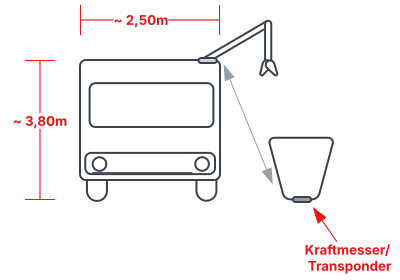
\includegraphics[scale=0.6]{aufgabe 3/img/dimensionen.svg}
    \caption{Typische Dimensionen eines Müllfahrzeuges. Je nach Montageposition der Leser/Transponder lassen sich die benötigten Frequenzen ableiten (Quelle: eigene)}
    \label{fig:dimensionen}
\end{figure}